\section{Introduction}
\label{sec:introduction}

The rapid advancement of Large Language Models (LLMs) has demonstrated remarkable capabilities in individual inference and generation tasks \citep{ai2023gpt, touvron2023llama, liu2024deepseek}. 
However, as the scale and complexity of real-world problems continue to grow, a fundamental bottleneck has emerged: the limited context window of a single model restricts its ability to process global information \cite{li2024loogle,chen2024long,an2024eval}. 
Even with recent progress in extending context lengths to millions of tokens \citep{reid2024gemini}, the quadratic cost of attention \citep{ratner2023parallel, yen2024long} makes centralized processing increasingly impractical for truly large-scale tasks.

\begin{figure}[t]
\vspace{1.0em} 
\centering
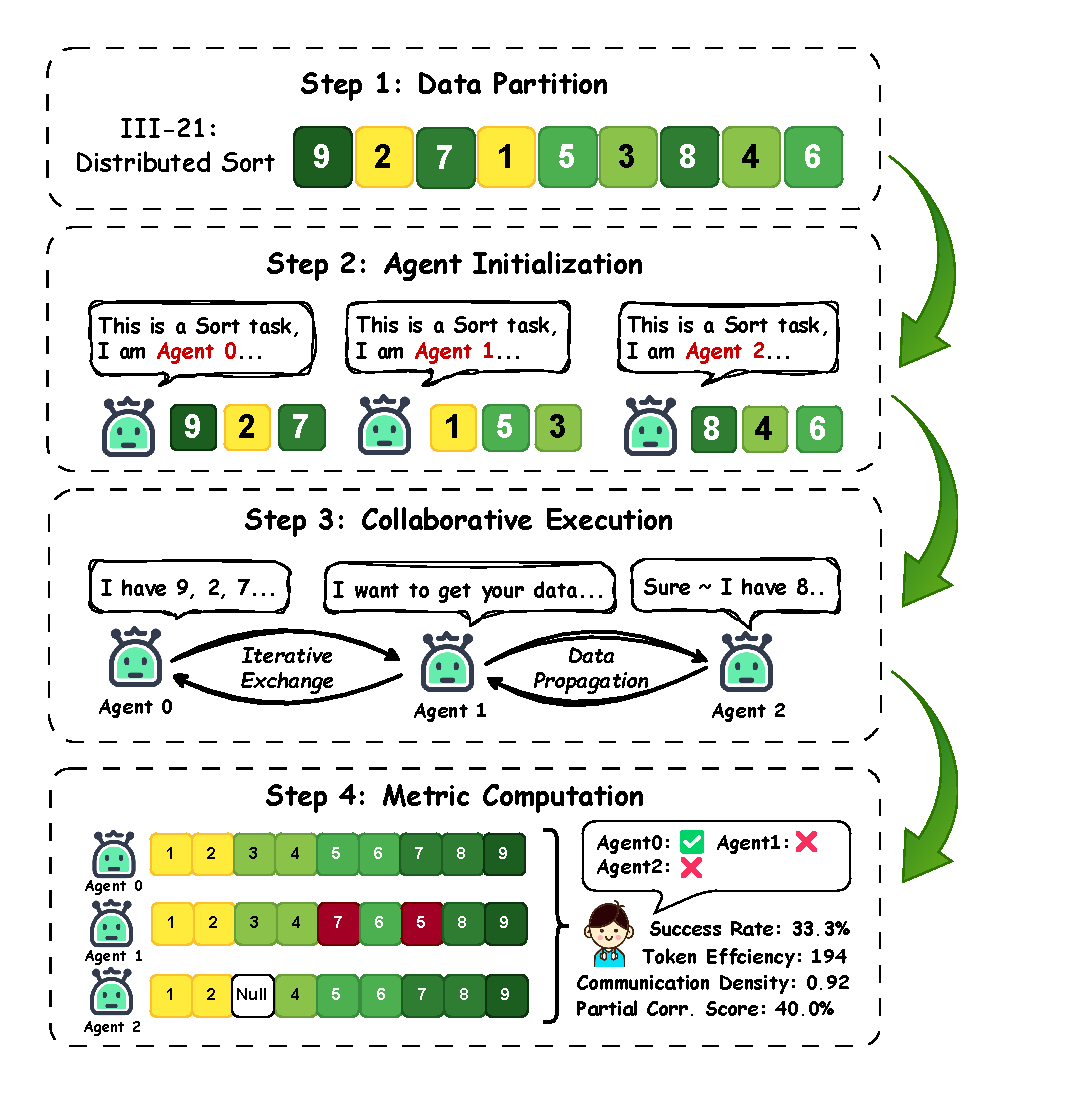
\includegraphics[width=1.0\columnwidth]{figures/figure1_overview_arxiv.pdf}
\caption{Pipeline of \silobench{}. Global information is partitioned across \(N\) agents, each holding only local data. Agents must communicate through the provided protocol to reconstruct global truth. Success requires effective collaboration strategies. This is an example of the III-21 Distributed Sort (Appendix \ref{app:tasks}.)}
\label{fig:overview}
\end{figure}

Multi-Agent Systems (MAS) offer a compelling architectural paradigm to address this scalability challenge \citep{zhang2024exploring, wang2024rethinking}. 
By distributing global information across multiple agents that collaborate to compute results, MAS can theoretically overcome the token limitations of single models \cite{liuagentbench}. 
This distributed approach mirrors successful patterns in traditional computing, from MapReduce to modern distributed databases, where data partitioning and coordinated computation across nodes achieve scales unattainable by a single machine \cite{dean2008mapreduce}. 
In the realm of large models, we define the scenario where an individual agent has access only to partial information, thereby necessitating coordination to resolve token constraints, as information silos. 
However, a critical question remains underexplored: Can current LLM-based agents effectively collaborate within information silos to compute a globally correct answer \cite{qian2024chatdev,qian2023communicative,liuagentbench}? 
Existing multi-agent benchmarks either prescribe fixed communication structures \citep{li2023camel, wu2024autogen, hong2023metagpt} or focus on social simulation rather than computational collaboration \citep{park2023generative, lan2024llm}. 
These approaches often introduce inductive bias into the agents' final outputs \citep{baltaji2024conformity}. 
For instance, if an agent is assigned the role of a "doctor", it may exhibit poor performance in artistic domains, which contradicts the goal of developing general-purpose agents \cite{an2024eval,qian2024chatdev,qian2023communicative,liuagentbench}. 
Furthermore, most benchmarks to date target specific tasks \citep{deng2024mobile, chen2024llmarena, gioacchini2024agentquest} and fail to address a significant gap in our understanding: whether logic-based models can autonomously discover and execute effective coordination strategies for distributed computing problems. 
Addressing this gap is a key objective for future AGI evaluation. 
To bridge this gap, we propose \silobench{}—a pioneering benchmark for evaluating free-form communication and collaboration in multi-agent LLM systems \cite{liuagentbench}. 
In summary, our contributions are as follows:
\begin{itemize}[leftmargin=*]
\item \textbf{We introduce \silobench{}, a role-agnostic configurable environment for evaluating distributed coordination under information silos.} 
Unlike static test suites that prescribe fixed roles and communication scripts, our framework can generate unlimited evaluation instances while providing high-level task hints and allowing observation of whether agents can translate structural understanding into effective coordination protocols \cite{presstrain,liuagentbench}. 
\item \textbf{We conduct the largest systematic study of multi-agent collaboration to date by instantiating 54 representative configurations.} 
Spanning diverse protocols and computing paradigms \citep{zhao2024electoral, islam2024mapcoder}, we propose a multi-dimensional metric suite to comprehensively quantify the trade-off between task success rate, token consumption, and communication density.
\item \textbf{We expose critical scalability limitations and the \emph{Communication-Reasoning Gap} in current LLMs.} 
Our results reveal that while agents can spontaneously discover task-appropriate communication topologies, they fail to translate effective coordination into correct distributed computation. 
This disconnection, coupled with inefficient information synthesis, causes performance to collapse as task complexity increases and the agent scale expands.
\end{itemize}
